\documentclass[10pt]{article}
\usepackage{natbib}
\usepackage{times}
\usepackage[T1]{fontenc}
\usepackage[utf8]{inputenc}
\usepackage[pdftex]{graphicx}
\usepackage{caption}
\captionsetup[figure]{justification=raggedright,labelfont=bf}
\usepackage{fullpage} % 1" margins
\usepackage{setspace}
\setstretch{1.5}
\usepackage{tabu}
\usepackage{xcolor}
\usepackage[backgroundcolor=yellow!30,bordercolor=yellow!30,textsize=small,textwidth=4cm]{todonotes}
\usepackage[unicode=true,colorlinks=true,urlcolor=blue,citecolor=black]{hyperref}
% \usepackage[top=2.5cm, bottom=2.5cm, outer=6cm, inner=1cm, heightrounded, marginparwidth=5cm, marginparsep=1cm]{geometry}
\usepackage[letterpaper,left=1.5cm,right=5cm]{geometry}
%\usepackage{sectsty}
%\sectionfont{\nohang\centering\normalsize\sc}   % capitalize initial letters
%\subsectionfont{\nohang\centering\normalsize\rm\em}

\renewcommand{\thetable}{S\arabic{table}}

% eat the colon so figures are labeled but have blank captions
% \makeatletter
% \renewcommand\fnum@figure[1]{\figurename~\thefigure\ignorespaces}
% \makeatother

\newcommand{\smalltodo}[2][]
{\todo[caption={#2}, size=\small, #1]
{\begin{spacing}{0.5}#2\end{spacing}}}

\newcommand{\fntodo}[2][]
{\todo[caption={#2}, size=\footnotesize, #1]
{\begin{spacing}{0.5}#2\end{spacing}}}

%% Article
\begin{document}
\raggedright
\parindent 0.5in


\begin{table}%[tbhp]
  \centering
  \small
  \caption{Global and regional sampling of clades.}
  \begin{tabu} to \textwidth {X[-3,l,b]|X[-1,r,b]X[-1,r,b]X[-1,r,b]|X[-1,r,b]X[-1,r,b]X[-1,r,b]|X[-1,r,b]X[-1,r,b]X[-1,r,b]|X[1,r,b]X[1,r,b]X[1,r,b]}
   \hline
    & \multicolumn{3}{c|}{global} & \multicolumn3{c|}{Hengduan Mountains} & \multicolumn3{c|}{Himalayas-QTP} & \multicolumn3{c}{temperate/boreal East Asia}\\
   clade                                                  & total & sampled & \% & total & sampled & \% & total & sampled & \% & total & sampled & \%  \\
   \hline
   \textit{Acer}                                          & 129   & 118     & 91 & 45    & 29      & 64 & 24    & 15      & 63 & 80    & 72      & 90  \\
   \textit{Allium}                                        & 800   & 378     & 47 & 34    & 29      & 85 & 55    & 37      & 67 & 89    & 100     & 89  \\
   Clematidinae+ Anemoninae                               & 495   & 177     & 36 & 76    & 32      & 42 & 45    & 26      & 58 & 152   & 72      & 47  \\
   Delphineae                                             & 756   & 312     & 41 & 225   & 74      & 33 & 83    & 44      & 53 & 90    & 51      & 57  \\
   \textit{Cyananthus}                                    & 66    & 47      & 71 & 41    & 28      & 68 & 26    & 24      & 92 & 14    & 10      & 71  \\
   \textit{Isodon}                                        & 100   & 63      & 63 & 55    & 40      & 73 & 20    & 9       & 45 & 36    & 24      & 67  \\
   \textit{Ligularia- Cremanthodium- Parasenecio} complex & 380   & 75      & 20 & 152   & 60      & 39 & 62    & 12      & 19 & 148   & 27      & 18  \\
   \textit{Meconopsis}                                    & 54    & 47      & 87 & 25    & 22      & 88 & 36    & 34      & 94 & 2     & 2       & 100 \\
   Microsoroideae                                         & 248   & 147     & 59 & 45    & 42      & 93 & 38    & 35      & 92 & 80    & 66      & 83  \\
   Pinaceae                                               & 234   & 226     & 97 & 34    & 32      & 94 & 26    & 24      & 92 & 63    & 63      & 100 \\
   Polygoneae                                             & 663   & 257     & 39 & 92    & 61      & 66 & 85    & 75      & 88 & 160   & 127     & 79  \\
   Primulaceae                                            & 900   & 354     & 39 & 205   & 114     & 56 & 150   & 68      & 45 & 80    & 55      & 69  \\
   \textit{Rhodiola}                                      & 70    & 57      & 81 & 32    & 28      & 88 & 37    & 30      & 81 & 34    & 20      & 59  \\
   \textit{Rhododendron}                                  & 1000  & 351     & 35 & 237   & 120     & 51 & 124   & 42      & 34 & 300   & 105     & 35  \\
   \textit{Rosa}                                          & 175   & 102     & 58 & 49    & 27      & 55 & 29    & 20      & 69 & 64    & 35      & 55  \\
   \textit{Saussurea}                                     & 416   & 147     & 35 & 108   & 73      & 68 & 130   & 63      & 48 & 157   & 56      & 36  \\
   Saxifragaceae+ Grossulariaceae                         & 760   & 313     & 41 & 209   & 54      & 26 & 155   & 45      & 29 & 170   & 102     & 60  \\
   \textit{Thalictrum}                                    & 150   & 104     & 69 & 38    & 34      & 89 & 40    & 25      & 63 & 48    & 32      & 67  \\
   \hline
    
  \end{tabu}
\end{table}

%%% Local Variables: 
%%% mode: latex
%%% TeX-master: "SI"
%%% End: 


\clearpage
\newpage

\section*{Materials and Methods}

\subsection*{Molecular dating: calibrations and topological constraints}

% \noindent We followed three general guidelines in calibrating the
% divergence-time analyses with node age constraints. All were intended
% to be conservative with respect to constraining the maximum age of any
% given clade.

% \begin{enumerate}

% \item We used the earliest confirmed fossil record of a group to
%   constrain its minimum \textit{stem} age; most fossil species are
%   published based on fragmentary material that lack enough characters
%   to be placed within the crown group.

% \item We applied uniform priors to all calibrations.% , despite the
%   % effect of inferred node age confidence intervals being larger than
%   % for other commonly-used distributions, e.g.\ lognormal, exponential,
%   % etc. We believe current knowledge on fossils only allow us to make
%   % an assumption that one clade could originate at any time between the
%   % minimum and maximum bounds.

% \item We used 125 Myr, the age of the earliest eudicot fossil
%   \citep{Hughes1994}, to constrain the maximum age of angiosperm
%   clades in the absence of other evidence.
% \end{enumerate}

Below we list and explain the node age constraints used in calibrating
the divergence-time analyses in BEAST. For each analysis, the ingroup
is the taxon for which divergence times and ancestral geographic
ranges were reconstructed; the ``outgroup scope'' is the
least-inclusive taxon containing the ingroup and outgroup taxa. Unless
otherwise noted, the age ranges are the bounds of a uniform prior
distribution, and the nodes in question were topologically constrained
to be monophyletic.

\subsubsection*{Clade \fntodo{what do clade numbers refer to? can we remove them?}1. Ingroup: \textit{Allium}; outgroup scope: Amaryllidaceae}

% \todo[inline]{Need a spreadsheet showing the taxa and genes (accession
%   numbers) used for each BEAST analysis}

% \todo[inline]{Need to add information about topological constraints in
%   addition to age constraints}

\noindent There are no reliable fossils for Amaryllidaceae, so we used
secondary calibrations from a fossil-calibrated study of the
containing order Asparagales \citep{Chen2013}.

\begin{enumerate}

\item \textbf{Root (crown age of Amaryllidaceae):} 42.0--61.7 Ma. The
  bounds equal the 95\% highest posterior density (HPD) interval of
  the crown age of Amaryllidaceae from \cite{Chen2013}.

\item \textbf{Crown age of Allioideae:} 27.8--44.5 Ma. The bounds
  equal the 95\% HPD interval of the crown age of Allioideae from
  \cite{Chen2013}.\fntodo{Was Allioideae constrained monophyletic?}

\end{enumerate}

\subsubsection*{Asteraceae}

We estimated a dated backbone phylogeny of Asteraceae for the purpose
of driving secondary calibrations for clade 2, the
\textit{Ligularia-Cremanthodium-Parasenecio} complex, and clade 3,
\textit{Saussurea}, both of which lack fossils. The backbone tree
included 499 genera of Asteraceae and four outgroup genera of
Calyceraceae (SI REF)\fntodo{provide this table of taxa x genes}. Each
genus was represented by one species. We calibrated the analysis using
the following node-age constraints.

% ?? calibrations as table?
% columns: clade, node, distribution--e.g. uniform(x, y), reasoning -
% explain how the distribution was derived, with reference to fossils
% or secondary calibrations, etc.

\begin{enumerate}

\item \textbf{Crown age of Asteraceae:} 72.1--125 Ma. The lower bound
  is based on Cretaceous pollen of \textit{Tubulifloridites lilliei}
  type A, which was used to constrain of the divergence time of
  \textit{Barnadesia} and \textit{Dasyphyllum} in
  \cite{Barreda2015}.

\item \textbf{Stem age of Asteraceae excluding Barnadesieae and
    \textit{Famatinanthus}:} 47.5--125 Ma. The lower bound is based
  on \textit{Raiguenrayum cura}, an exceptionally well-preserved
  capitulescence from the 47.5 Ma Huitrera Formation in Argentina
  \citep{Barreda2010,Barreda2012} that shares a mosaic of
  morphological characters with modern groups such as Stifftieae,
  Mutisioideae sensu lato, and Carduoideae.

\item \textbf{Stem age of Mutisieae:} 28.5--125 Ma. The lower bound
  is based on the earliest unequivocal fossil pollen for Mutisieae,
  \textit{Mutisiapollis patersonii}, from the early Oligocene of
  Australia \citep{Macphail1994}. The pollen is similar to that of
  some extant species in \textit{Chaetanthera} and \textit{Mutisia},
  however, it cannot be clearly placed within any extant genus.

\item \textbf{Stem age of Nassauvieae:} 16.0--125 Ma. The lower
  bound was set by the earliest fossil pollen of Nassauvieae,
  \textit{Huanilipollis cabrerii}, from early Miocene sediments in
  South America \citep{Barreda2008,Barreda2010}. It is similar to
  pollen of recent \textit{Holocheilus}, \textit{Jungia}, and
  \textit{Proustia}, being subprolate, tricolporate, microechinate and
  with a complex exine structure \citep{Barreda2008}.

\item \textbf{Stem age of Cichorieae excluding Scorzonerinae:}
  22.0--125 Ma. The lower bound is based on the earliest confirmed
  fossil pollen of Cichorieae, \textit{Cichorium intyubs}-type pollen
  from the Molasse of the Paratethys, which is at least 22 Ma old
  \citep{Hochuli1978}. The pollen has three poral lacunae, six abporal
  lacunae (three at each side of the equator), and six paraporal
  lacunae (three on each side of the equatorial ridge)
  \citep{Blackmore1984}, a trait combination widely distributed in all
  subtribes except Scorzonerinae \citep{Tremetsberger2013}.

\item \textbf{Stem age of \textit{Sonchus} + \textit{Launaea}:}
  5.4--125 Ma. The lower bound is based on \textit{Sonchus
    oleraceus}-type pollen from the Late Miocene, which resembles that
  of extant \textit{Aetheorhiza}, \textit{Hyoseris}, \textit{Launaea},
  and \textit{Sonchus} \citep{Blackmore1986}. Our sampling included
  only the latter two genera.

\end{enumerate}

\noindent We used 95\% HPD intervals for node ages in the backbone
tree as secondary calibrations for the
\textit{Ligularia-Cremanthodium-Parasenecio} complex and
\textit{Saussurea} as described below.

\subsubsection*{Clade 2. \textit{Ligularia-Cremanthodium-Parasenecio} complex}

\begin{enumerate}

\item \textbf{Root age:} 9.5--29.8 Ma.

\item \textbf{Crown age of \textit{Ligularia}:} 2.32--16.85 Ma.

\item \textbf{Crown age of \textit{Petasites} + \textit{Tussilago}}:
  1.09--15.18 Ma.

\end{enumerate}

\subsubsection*{Clade 3. \textit{Saussurea}}

\begin{enumerate}
\item \textbf{Root age:} 2.27--13.98 Ma. % INGROUP??
\end{enumerate}

\subsubsection*{Clade 4. Ingroup: \textit{Cyananthus}; outgroup scope: Campanulaceae}

\begin{enumerate}

\item \textbf{Root (crown age of Campanulaceae):} 62--90 Ma. The
  bounds equal the 95\% HPD interval of the crown age of Campanulaceae
  inferred in \cite{Magallon2015}.

\item \textbf{Stem age of the most recent common ancestor of
    \textit{Campanula pyramidalis} and \textit{C.~carpatica}:} 16.5--62
  Ma. The bounds are based on fossils of \textit{C.~palaeopyramidalis}
  \citep{Lancucka-Srodoniowa1979} which were evaluated as belonging to
  \textit{C. pyramidalis} in \cite{Cellinese2009}.
\end{enumerate}

\subsubsection{Clade 5. Ingroup: \textit{Rhodiola}; outgroup context:
  Crassulaceae}

As no reliable fossils are available for Crassulaceae, we estimated
divergence times in \textit{Rhodiola} in the context of
Saxifragales. One hundred and seventy-one species from the
Saxifragales were selected as outgroups. We applied the same fossil
calibrations as Saxigragaceae and Grossulariaceae (detailed
information see fossil calibrations for Saxifragaceae and
Grossulariaceae).

\subsubsection{Clade 6. Ingroup: \textit{Rhododendron}; outgroup context: Ericaceae}

\smalltodo[inline]{This paragraph needs to be more clear}

{\color{red}To incorporate more fossil calibrations, we selected several species
from Empetrum, Enkianthus, Erica and Kalmia as outgroups.  We mainly
use fossil calibrations for Ericaceae selected by Schwery et
al. \citep{Schwery2015}. However, to be more conservative, we
constrained the stem age rather than the crown age of Rhododendron
using the earliest fossil of this genus. This because the earliest
fossil cannot be assigned to any subgenus based on morphological
characters. We applied the earliest fossil record of Ericaceae (89.8
Myr) to be the maximum age of other calibrations in the Ericaceae.}

\begin{enumerate}

\item \textbf{Root (crown age of Ericaceae):} 89.8--125 Ma. The
  lower bound is based on the earliest fossil record of Ericaceae,
  \textit{Paleoenkianthus sayrevillensis} \citep{Nixon1993}.

\item \textbf{Stem age of \textit{Rhododendron}:} 56--89.8 Ma. The
  lower bound is the earliest fossil record of the genus,
  \textit{R.~newburyanum} from the Paleocene of South England
  \citep{Collinson1978}. The maximum is from constraint 1.

\item \textbf{Stem age of \textit{Erica}:} 5.33--89.8 Ma. The lower
  bound is based on the earliest fossil record of the genus,
  \textit{E.~palaeoarborea} from the late Miocene of Europe
  \citep{VanderBurgh1987}. The maximum is from constraint 1.

\item \textbf{Stem age of \textit{Empetrum}:} 11.62--89.8 Ma. The
  lower bound is based on the earliest fossil record of the genus,
  from the middle Miocene of Denmark \citep{Friis1979}. The maximum is
  from constraint 1.

\item \textbf{Stem age of \textit{Kalmia}:} 15.97--89.8 Ma. The lower
  bound is based on the earliest fossil record of the genus,
  \textit{K.~saxonica} from the early Miocene of Germany
  \citep{VanderBurgh1987}. The maximum is from constraint 1.

\end{enumerate}

\subsubsection*{Clade 7. Ingroup: \textit{Isodon}; outgroup context:
  Lamiaceae}

\smalltodo[inline]{Was our sampling different? Why not use the fossils
  directly, instead of secondary calibrations?}

{\color{red}Divergence times for \textit{Isodon} were estimated using fossil
calibrations by \citet{Yu2014}. We used 95\% HPD intervals from that
study to calibrate 2 nodes in our analysis.}

\begin{enumerate}
\item \textbf{Stem age of \textit{Isodon}:} 17.03--39.84 Ma.
\item \textbf{Crown age of \textit{Isodon}:} 14.66--26.44 Ma.
\end{enumerate}

\subsubsection*{Clade 8. Ingroup: \textit{Meconopsis}; outgroup
  context: Papaveraceae}

\begin{enumerate}
\item \textbf{Crown age of \textit{Meconopsis}:} 12--34 Ma. The bounds
  are based on the 95\% HPD interval for the node estimated in a study
  by \citet{Xiao2013}, which used fossil calibrations from other taxa
  in Ranunculales.
\end{enumerate}

\subsubsection*{Clade 9. Pinaceae}

\begin{enumerate}
\item \textbf{Root (crown age of Pinaceae):} 152--200 Ma. The lower
  bound is based on the earliest fossil cone assigned to Pinaceae,
  \textit{Eathiestrobus} \citep{Rothwell2012}. The maximum bound was
  set to 200 Ma based on the absence of Pinaceae fossils before the
  Jurassic.%  We placed three fossil calibrations in Pinaceae selected
  % by Leslie et al. \citep{Leslie2012}. We also followed their settings
  % of the lower and upper bounds \citep{Leslie2012}, but use uniform
  % priors.

\item \textbf{Stem age of \textit{Larix}:} 41--60 Ma. The bounds
  follow \citet{Leslie2012}. The lower bound is based on the
  earliest reliable fossil of \textit{Larix}, \textit{L.~altoborealis}
  from the middle Eocene of Canada \citep{LePage1991}.

\item \textbf{Stem age of Picea:} 133--153 Ma. The bounds follow
  \citet{Leslie2012}. The lower bound is based on \textit{Picea
    burtonii}, the earliest reliable fossil of \textit{Picea} from the
  Early Cretaceous Apple Bay locality in British Columbia
  \citep{Klymiuk2012}.

\item \textbf{Stem age of Tsuga:} 41--100 Ma. The bounds follow
  \citet{Leslie2012}. The lower bound is based on \textit{Tsuga
    swedaea} from the middle Eocene Buchanan Lake formation, Axel
  Heiberg Island \citep{Lepage2003}.

\end{enumerate}

\subsubsection*{Clade 10. Ingroup: Polygoneae; outgroup context:
  Polygonaceae}

\begin{enumerate}

\item \textbf{Root (stem age of Polygonaceae):} 65.5--125 Ma. The
  lower bound is based on the fossil fruit \textit{Polygonocarpum
    johnsonii} from the Maastrichtian of North Dakota, which exhibits
  wing venation patterns known only in Polygonaceae
  \citep{Manchester2010}.

\item \textbf{Stem age of \textit{Polygonum}:} 28.1--125 Ma. The
  lower bound is based on the earliest fossil record of
  \textit{Polygonum} from the early Oligocene of western Siberia
  \citep{Dorofeev1963}.

\item \textbf{Stem age of \textit{Persicaria}:} 55.8--125 Ma. The
  lower bound is based on several \textit{Persicaria}-type pollen
  fossils reported from the Paleocene of Europe
  \citep{Krutzsch1970,Gruas1978} and accepted by \citet{Muller1981}.

\item \textbf{Stem age of \textit{Rumex}:} 16--125 Ma. The lower
  bound is based on seed and fruit fossils of the genus from the
  middle Miocene of Germany \citep{Mai2001}.

\item \textbf{Crown age of \textit{Muehlenbeckia}:} 12.7--125 Ma. The
  lower bound is based on the 12.7 Ma fossil of the extant species
  \textit{M.~australis} from New Zealand
  \citep{Pole1993,Schuster2013}.

\end{enumerate}

\subsubsection*{Clade 11. Ingroup: Microsoroideae; outgroup context:
  Polypodiaceae}

% One hundred and seventy-nine species from Polypodiaceae were selected
% as outgroups.

\begin{enumerate}
\item \textbf{Root (crown age of Polypodiaceae):} 33.9--77 Ma. The
  lower bound is based on the earliest uncontroversial fossil of
  Polypodiaceae, \textit{Protodrynaria takhtajanii} from the Eocene of
  Siberia \citep{Vikulin1987}. The maximum bound is based on a
  secondary calibration, the upper bound of the 95\% HPD for the crown
  age of polygrammoids \citep{Schuettpelz2009}.

\item \textbf{Crown age of \textit{Drynaria}:} 5.3--66 Ma. The lower
  bound is based on a fossil of the extant species
  \textit{D.~propinqua} from the late Miocene of SW China
  \citep{Wen2013}. The upper bound is based on the assumption that the
  genus is unlikely to have originated before the Cenozoic.

\item \textbf{Stem age of \textit{Polypodium}:} 25.6--66 Ma. The
  lower bound is based on the earliest fossil record of the genus
  from the early Oligocene of Czech Republic \citep{Kvacek2001}. The
  upper bound is based on the assumption that the genus is unlikely to
  have originated before the Cenozoic.

\item \textbf{Stem age of Pleopeltis:} 15.8--66 Ma. The lower bound
  is based on the oldest reliable fossil of the genus, from the
  Miocene of the Dominican Republic \citep{Schneider2015}. The upper
  bound is based on the assumption that the genus is unlikely to have
  originated before the Cenozoic.
\end{enumerate}

\subsubsection*{Clade 12. Ingroup: Primuloideae; outgroup context:
  Primulaceae s.~l.}

% We expanded our sampling to the whole Primulaceae (s. l.). Five
% fossils were used as calibrations in dating the Primulaceae
% phylogeny. 

\begin{enumerate}
\item \textbf{Root (crown age of Primulaceae s.~l.):} 48.6--72 Ma. The
  lower bound is based on the earliest fossil record of the
  Primulaceae s.~l., from the early Eocene London Clay Formation and
  assigned to \textit{Ardisia} \citep{Collinson1984}. Fossils of
  Myrsinoideae have also been reported from the early Eocene United
  States \citep{Irving1971}. The maximum bound is based on the
  earliest fossil flowers of {\color{red}the Primuloids} \fntodo{what
    is this group?} from the Late Cretaceous (Campanian-Maastrichtian)
  Mira locality of Portugal \citep{Friis2011}.

\item \textbf{Stem age of Primuloideae (Primulaceae s.s.):} 28--72
  Ma. The lower bound is based on the earliest fossils of
  Primuloideae, from the early Oligocene of Siberia
  \citep{Nikitin2006}. {\color{red}The maximum bound follows
    constraint 1.}

\item \textbf{Stem age of \textit{Primula}:} 15.96--72 Ma. The lower
  bound is based on the earliest unequivocal fossil of
  \textit{Primula}, \textit{P.~riosiae}
  \citep{deVos2014}. {\color{red}The maximum bound follows constraint
    1.}

\item \textbf{Stem age of \textit{Androsace}:} 5.3--72 Ma. The lower
  bound is based on the earliest fossil seed of \textit{Androsace},
  from the Miocene of western Siberia \citep{Dorofeev1963}.
\end{enumerate}

\subsubsection*{Ingroups: Delphineae, \textit{Clematis}, and
  \textit{Thalictrum}; outgroup context: Ranunculaceae}

The fossil record of Ranunculaceae has been reviewed by
\citet{Friis2011} and \citet{Pigg2005}. The Cretaceous record of the
Ranunculaceae is sparse. For Delphinea, we expanded our sampling to
the whole Ranunculaceae. One hundred and thirty-eight species from
other genera of Ranunculaceae were selected as outgroups.

\begin{enumerate}
\item \textbf{Root (crown age of Ranunculaceae):} 93.9--125 Ma. The
  lower bound is based on pollen of \textit{Cretacaeisporites
    scabratus} from the Cretaceous (probably Late Cenomanian) of Gabon
  \citep{Ward1994}.

\item \textbf{Stem age of \textit{Actaea}:} 56.8--125 Ma. The lower
  bound is based on fossil fruits (\textit{Paleoactaea nagelii}) from
  the late Paleocene of North Dakota \citep{Pigg2005}.

\item \textbf{Stem age of \textit{Clematis}:} 23--125 Ma. The lower
  bound is based on fossil fruits of the genus from the Oligocene of
  Germany \citep{Weyland1938}.

\item \textbf{Stem age of \textit{Caltha}:} 70.6--125 Ma. The lower
  bound is based on fossil \textit{Eocaltha zoophilia} from the
  Campanian of Mexico \citep{Rodriguez1998}.

\item \textbf{Stem age of \textit{Ranunculus}:} 23--125 Ma. The
  lower bound is based on fossil fruits of the genus from the
  Oligocene \citep{Mai1985}.

\end{enumerate}

% We applied all fossil calibrations used for the Delphinae in dating
% Clematidinae-Anemoninae and Thalictroideae. Besides above fossil
% calibrations, we added two more calibrations. We used Eocaltha
% zoophilia from the Campanian of Mexico which show similarity to seeds
% of extant Caltha to constrain the stem age of Caltha
% \citep{Rodriguez1998}. The stem age of Caltha was set to 70.6--125
% Myr. We applied the Oligocene Ranunculus fossil fruits to constrain
% the stem age of this genus \citep{Mai1985}. The stem age of Ranunculus
% was set to 23--125 Myr.

\subsubsection*{Clade 16. Ingroup: \textit{Rosa}; outgroup context:
  Rosaceae}

% Rosales has very good fossil record among all the angiosperms
% \citep{Xing2016}. To incorporate more fossil calibrations, we selected
% 203 taxa from other genera of Rosaceae and four species of Rhamnaceae
% as outgroup.

\begin{enumerate}
\item \textbf{Root (age of split between Rosaceae and Rhamnaceae):}
  70--125 Ma. The lower bound is based on the oldest fossil flower
  of Rhamnaceae, \textit{Coahuilathus belindae}, from the late
  Campanian of Mexico \citep{Calvillo-Canadell2007}.

\item \textbf{Crown age of subfamily Spiraeoideae excluding
    \textit{Lyonothamnus}, supertribe Kerriodae, and tribe Neilieae):}
  49.4--125 Ma. The lower bound is based on the earliest fossil of
  Spiraeoideae, \textit{Paleorosa} from the middle Eocene of British
  Colombia \citep{Basinger1976}.

\item \textbf{Crown age of Amygdaleae:} 49.4--125 Ma. The lower
  bound is based on a fossil of \textit{Prunus} from the middle Eocene
  \citep{DeVore2007}.

\item \textbf{Crown age of tribe Kerriae:} 49.4--125 Ma. The lower
  bound is based on the earliest fossil record for the tribe, assigned
  to the genus \textit{Neviusia}, from the middle Eocene of British
  Columbia \citep{DeVore2004}.

\item \textbf{Stem age of Rosa:} 34--125 Ma. The lower bound is
  based on the earliest fossil record of the genus, from the late
  Eocene Florissant Formation \citep{Manchester2001}.
\end{enumerate}

\subsubsection*{Clade 17. Ingroup: \textit{Acer}; outgroup context:
  Sapindaceae}

The analysis included 118 ingroup species and 2 outgroups,
\textit{Dipteronia dyeriana} and \textit{D.~sinensis}.

\begin{enumerate}

\item \textbf{Stem age of \textit{Dipteronia}:} 60--125 Ma. The
  lower bound is based on the earliest fossil of
  \textit{Dipteronia}, winged fruits from the Paleocene of North
  America \citep{McClain2001}.

\item \textbf{Crown age of Acer:} 47.8--125 Ma. \textit{Acer} has a
  rich fossil record, dating to at least the Paleocene
  \citep{Wolfe1987,Mai1995}. We based the lower bound on the crown
  age on the first fossil samaras assignable to \textit{Acer} section
  \textit{Acer}, from the latest Early Eocene of North America
  \citep{Wolfe1987}.

\end{enumerate}

\subsubsection*{Clade 18: Ingroup: Saxifragaceae + Grossulariaceae;
  outgroup context: Saxifragales}

The analysis included 313 ingroup species and five species of
\textit{Itea} and one species of \textit{Pterostemon} as outgroups.

\begin{enumerate}
\item \textbf{Root age (crown Saxifragales):} 90--125 Ma. The lower
  bound is based on the Turonian fossil \textit{Divisestylus}, which
  shows flowers and fruits with well-preserved morphological
  characters that indicate a clear affinity to Iteaceae
  \citep{Hermsen2003}.

\item \textbf{Stem age of \textit{Itea}:} 49--125 Ma. The lower
  bound is based on the earliest fossil pollen assigned to \emph{Itea}
  \citep{Hermsen2013}.

\item \textbf{Stem of Ribes:} 42--125 Ma. The lower bound is based
  on the earliest uncontroversial fossil leaves assigned to
  \textit{Ribes axelrodii} from the Eocene Bull Run floras
  \citep{Hermsen2005}.
\end{enumerate}

\subsection*{Biogeographical range scoring}

Data matrices for the geographic ranges of species sampled in the
studies clades were assembled mainly based on the online eFloras and
databases such as
\href{http://www.efloras.org/flora_page.aspx?flora_id=2}{Flora of
  China}, \href{http://floranorthamerica.org}{Flora of North America},
\href{http://www.efloras.org/flora_page.aspx?flora_id=5}{Flora of
  Pakistan}, \href{http://www.emplantbase.org}{EURO+MEDI PlantBase},
\href{http://plants.usda.gov}{USDA},
\href{http://www.efloras.org/flora_page.aspx?flora_id=110}{Annotated
  Checklist of the Flowering Plants of Nepal}, and
\href{http://www.gbif.org}{Global Biodiversity Information
  Facility}. We excluded records of introduced (non-native)
species. We obtained a county level distribution for most of
Himalayan-Hengduan region species by cross checking with Biodiversity
of the Hengduan Mountains database (http://hengduan.huh.harvard.edu),
dataset of distributions ranges for species included in Vascular
Plants of the Hengduan Mountains compiled by Zhang et
al. \citep{Zhang2009}, and Wu \citep{Wu2008}.

\subsection*{Ancestral regions reconstruction}

\bibliography{SI-refs}
\bibliographystyle{ecol_let}

% \begin{figure}
% \begin{center}
% 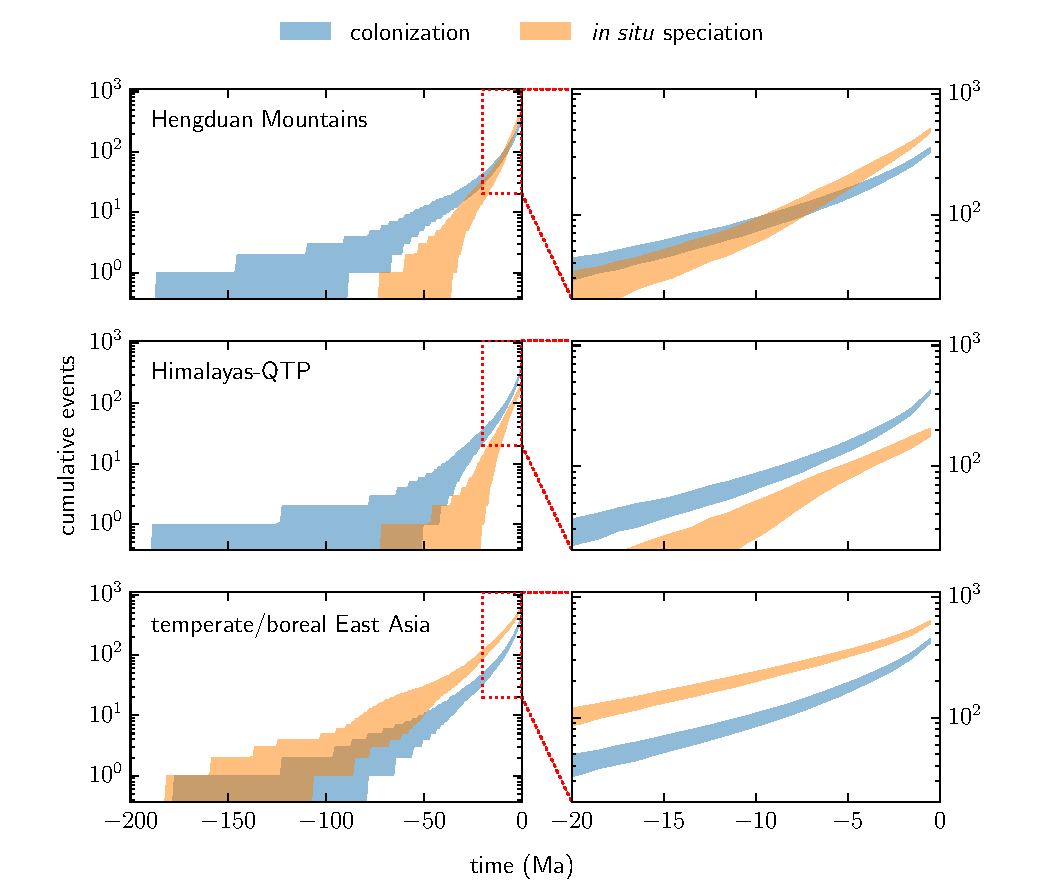
\includegraphics[width=.99\textwidth]{figures/figure_cumulative_events/figure_cumulative_events.pdf}
% \end{center}
% \caption{Assembly of regional floras by colonization and \textit{in situ} speciation events in 18 plant clades, inferred from ancestral-range reconstructions on time-calibrated molecular phylogenies. Shaded regions indicate the 5--95\% quantile intervals for the cumulative number of events through time from 500 pseudoreplicated joint biogeographic histories designed to account for phylogenetic uncertainty (see text). Panels on the right focus on the last 20 Ma, in which differences in regional assembly are most apparent. In the Hengduan Mountains region, cumulative \textit{in situ} speciation overtakes colonization about 8 Ma, whereas for the Himalayas-QTP, colonization remains the dominant process. \textit{In situ} speciation thus appears to have played a disproportionately large role in assembling the Hengduan Mountains flora since the late Miocene compared to the Himalayas-QTP, consistent with the theory of uplift-driven diversification in the Hengduan Mountains region.}
% \label{fig:cumevents}
% \end{figure}

\end{document}

%%% Local Variables:
%%% mode: latex
%%% TeX-master: t
%%% End:
